\section{Uczenie ze wzmocnieniem}

W uczeniu ze wzmocnieniem, agent działający w pewnym środowisku, podejmuje akcje, które mogą na nie oddziaływać. Po wykonaniu akcji, agent otrzymuję nagrodę, która stanowi miarę jakości jego działania. Cel agenta to maksymalizowanie otrzymywanych nagród, oznacza to, że agent musi nauczyć się dopasować akcje względem stanu, w którym się znajduje.

\begin{figure}[H]
	\centering
	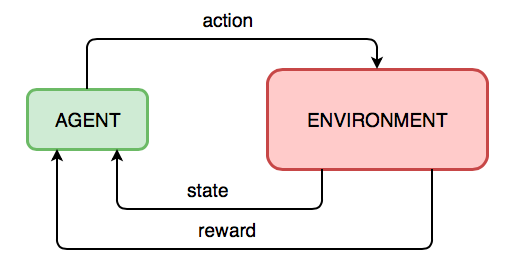
\includegraphics[width=0.7\linewidth]{imgs/rl}
	\caption{Schemat działania uczenia ze wzmocnieniem.}
	\label{fig:rl}
\end{figure}

Przy badaniach uczenia ze wzmocnieniem wykorzystano algorytm Q-learning. Polega on na tym, że dla stanu $s_{t}$ oraz pewnej wybranej akcji $a_{t}$ dla kroku $t$, w kolejnym stanie, wyznaczana jest wartość funkcji $Q(s_{t}, a_{t})$, według poniższej formuły.

$$Q(s_{t}, a_{t}) = (1 - \alpha) \cdot Q(s_{t}, a_{t}) + \alpha \cdot \Big( r_{t} + \gamma \cdot \max_{a} Q(s_{t + 1}, a) \Big)$$

Pozostałe oznaczenia:
\begin{itemize}
	\item $\alpha$ -- współczynnik uczenia (w jakim stopniu uwzględniać nagrodę za stary stan oraz ten nowy),
	\item $\gamma$ -- współczynnik uwzględniania przyszłych nagród.
\end{itemize}

Przy realizacji Q-learningu zdecydowano się na dwa podejścia w przyznawaniu nagród za wykonywane akcje w danym stanie:

\begin{itemize}
	\item co krok -- wartość Q dla każdej pary jest aktualizowana od razu, gdzie podczas gry każda z nich dostaje nagrodę zerową, tylko ostatnia para otrzymuje nagrodę $\pm 1$,
	\item co grę (batch mode) -- każda z par jest zapisywana, dopiero w momencie zakończenia gry, każda z tych par otrzymuje nagrodę.
\end{itemize}

Polityki wybierania akcji:
\begin{itemize}
	\item zawsze najlepsza (lepsza eksploitacja),
	\item eps-greedy -- określany jest parametr $\epsilon$, który oznacza prawdopodobieństwo wyboru losowej, a nie najlepszej akcji (lepsza eksploracja).
\end{itemize}

\pagebreak